% vim: set ai tw=80 fileencoding=utf8: 
%-------------------------------------------------------------------------------
\documentclass[
  % -- opções da classe memoir --
	12pt,				% tamanho da fonte
	openright,			% capítulos começam em pág ímpar (página vazia se preciso)
  %twoside,			% para impressão em verso e anverso. Oposto a oneside
  oneside,			% oposto de twoside, para nao gerar paginas 
	a4paper,			% tamanho do papel. 
	% -- opções da classe dc-uel --
	tcc,			% tipo do trabalho (opções: tcc, dissertacao, qualificacaoms)
	]{dc-uel}


% ---
% PACOTES
% ---
\usepackage{listings}
\usepackage{color}
\usepackage{morefloats}
\definecolor{red}{rgb}{0.6,0,0} % for keywords
\definecolor{green}{rgb}{0.25,0.5,0.35} % comments
\definecolor{purple}{rgb}{0.5,0,0.35} % strings
\definecolor{blue}{rgb}{0.25,0.35,0.75} % doc
 
\lstset{language=c,
basicstyle=\ttfamily,
keywordstyle=\color{red}\bfseries,
stringstyle=\color{purple},
commentstyle=\color{green},
morecomment=[s][\color{blue}]{/**}{*/},
numbers=left,
numberstyle=\tiny\color{black},
stepnumber=1,
numbersep=7pt,
tabsize=2,
showspaces=false,
showstringspaces=false}



% ---
% Pacotes fundamentais 
% ---
\usepackage[T1]{fontenc}		% Selecao de codigos de fonte.
\usepackage[utf8]{inputenc}		% Codificacao do documento
\usepackage{graphicx}			% Inclusão de gráficos
\usepackage[Algoritmo,plain]{algorithm}
\usepackage{algorithmic}
\usepackage{tikz}
\usetikzlibrary{arrows}

% numeração de figuras e tabelas considerando o capítulo (9.1 9.2)
\usepackage{amsmath}
\numberwithin{figure}{chapter}
\numberwithin{table}{chapter}
\numberwithin{algorithm}{chapter}
% ---
		
% ---
% Pacotes adicionais, usados apenas no âmbito do Modelo Canônico do abnteX2
% ---
\usepackage{lipsum}				% para geração de dummy text
% ---

% ---
% Informações de dados para CAPA, FOLHA DE ROSTO e outros elementos
% ---
\titulo{Otimização de codigo com técnicas de transformação de loops}
\tituloingles{Code otimization with loop transformations techiniques}
\palavraschave{otimizição.\ tranformação de loops.}
\palavraschaveingles{optmization.\ loops transformations.}
\autor{Luiz Guilherme Castilho Martins}
\citacaoautor{MARTINS, L. G. C.}
\data{2013}

\diadefesa{24 de novembro}
\orientador{Prof. Dr. Wesley Attrot} % É membro nato e presidente da Banca Examinadora
\membrobancadois{Prof. Dr. Segundo Membro da Banca}
\instmembrobancadois{Universidade Estadual de Londrina}
\membrobancatres{Prof. Msc. Terceiro Membro da Banca}
\instmembrobancatres{Universidade Estadual de Londrina}
% \membrobancaquatro{Prof. Esp. Quarto Membro da Banca}
% \instmembrobancaquatro{Universidade/Instituição do Quarto Membro da Banca}

% ---
% compila o indice
% ---
\makeindex
% ---

% ----
% Início do documento
% ----
\begin{document}

% Retira espaço extra obsoleto entre as frases.
\frenchspacing 

% ----------------------------------------------------------
% ELEMENTOS PRÉ-TEXTUAIS
 ----------------------------------------------------------
 \pretextual


  % vim: set ai tw=80 fileencoding=latin1: 
%-------------------------------------------------------------------------------

\thispagestyle{empty}
		\begin{figure}[htb]
					\centering \includegraphics[width=14cm]{1-capa/imagens/logo-uel.png}
		\end{figure}

		\begin{figure}[htb]
					\centering \includegraphics[scale=0.7]{1-capa/imagens/barra-capa.png}
		\end{figure}

		\begin{center}
            {\bf \large \nome }
    \end{center} 
    \vspace*{\stretch{4}}
				\begin{center}
                {\large \textbf {\titulotcc}} \\ \vspace{2ex}
				\end{center}

		\vspace*{\stretch{6}}

		\begin{figure}[htb]
				\centering \includegraphics[scale=0.7]{1-capa/imagens/barra-capa.png}
		\end{figure}

		\begin{center}
				{\tamanhonormal Londrina - PR \\ 2013}
		\end{center}

%  \input{1-capa/1-folha-de-rosto}
%  \input{1-capa/2-errata}
  % vim: set ai tw=80 fileencoding=utf8: 
%-------------------------------------------------------------------------------

\includepdf{folha-aprovacao}

  % vim: set ai tw=80 fileencoding=latin1: 
%-------------------------------------------------------------------------------


\newpage
\
\vfill
\begin{flushright}
		\hfill \textit{A todos aqueles que \\ 
                        me apoiaram e contribu�ram \\ 
                        para conclus�o deste trabalho.}
\end{flushright}
\vspace*{1cm}
\clearpage


  % vim: set ai tw=80 fileencoding=utf8: 
%-------------------------------------------------------------------------------
\begin{agradecimentos}
Agradeço primeiramente aos meus irmãos que estiveram por perto durante toda
a graduação e meus pais que me apoiaram e incentivaram 
em tudo e sempre.
        
Professor Dr. Wesley Attrot, que propôs este tema desafiador e me motivou e 
incentivou durante a realização deste trabalho.

Aos amigos: 
Arthur Coutinho que me ajudou muito neste e em outros desafios. 
Beatriz que todos temem. 
Breno Kusunoki que sempre diz que horas são.
Mateus Piveta. 
Clayton Kuwabara por ser mac fag. 
Hélio que me ensiou que não está fácil nem para ela. 
Randal que me ajudou a corrigir este trabalho e é bobo. 
Ernesto que adora harumaki.
E todos os amigos que fiz durante a graduação, todas as horas de estudo
e brincadeiras que tivemos juntos.

Agradeço a Bijuzinho, Gab, Morgana, Janja, Princesa Léia, e Maria, responsáveis
por momentos de descontração durante a graduação.

Todos os professores que de uma forma ou outra, muito me ensinaram.

Agredeço também todos os funcionários da UEL, que no exercício de suas funções,
ajudaram a tornar a graduação mais agradável.
\end{agradecimentos}

  % vim: set ai tw=80 fileencoding=latin1: 
%-------------------------------------------------------------------------------

\newpage
\
\vfill
\begin{flushright}
		%\hfill \textit{"texto da ep�grafe"} \\
		%{\bf autor da ep�grafe}
		\hfill \textit{"O importante � ganhar. Tudo e sempre. \\
                        Essa hist�ria que o importante � competir n�o passa de 
                        demagogia."} \\
        {\bf Ayrton Senna}
\end{flushright}
\vspace*{1cm}


  % vim: set ai tw=80 fileencoding=utf8: 
%-------------------------------------------------------------------------------
\begin{resumo}
        Paralelização de código permite ao programador a oportunidade de criar algoritmos para resolver problemas com maior eficiência.
        Programas são ditos paralelos quando existem duas ou mais ações executando simultaneamente em diferentes unidades de processamento.
        O objetivo deste trabalho é estudar técnicas de paralelização de código e tentar desenvolver uma nova otimização ou técnica de paralelização.
\end{resumo}

  % vim: set ai tw=80 fileencoding=utf8: 
%-------------------------------------------------------------------------------
\begin{Abstract}
 This is the english abstract. The Abstract in English should be faithful to the
 Resumo in Portuguese, but not a literal translation.
\end{Abstract}



% ---
% inserir lista de ilustrações
% ---
\pdfbookmark[0]{\listfigurename}{lof}
\listoffigures*
\cleardoublepage
 ---

%---
%inserir lista de tabelas
%---
\pdfbookmark[0]{\listtablename}{lot}
\listoftables*
\cleardoublepage
% ---

% vim: set ai tw=80 fileencoding=utf8: 
%-------------------------------------------------------------------------------
\begin{siglas}
        % C
        \item[CPU] Central Processing Unit

        % I
        \item[IW] Instruction Word 

        % M
        \item[MISD] Multiple Instruction Single Data
        \item[MIMD] Multiple Instruction Multiple Data

        % S
        \item[SISD] Single Instruction Single Data
        \item[SIMD] Single Instruction Multiple Data

        % V
        \item[VLIW] Very Long Instruction Word
\end{siglas}


%% vim: set ai tw=80 fileencoding=utf8: 
%-------------------------------------------------------------------------------
\begin{simbolos}
  \item[$ \delta $] Letra grega delta 
\end{simbolos}



 % ---
 %inserir o sumario
 %---
\pdfbookmark[0]{\contentsname}{toc}
\tableofcontents*
\cleardoublepage

\textual

% vim: set ai tw=80 fileencoding=utf8: 
%-------------------------------------------------------------------------------
\chapter{Introdução}

Diante da  dificuldade de se melhorar processadores \textit{single-core} devido ao alto consumo de energia e as altas
temperaturas, a indústria de processadores adotou como solução à esses
problemas, o desenvolvimento de processadores \textit{multi-core},
além disso também considerou-se o poder de processamento quando se utilizam vários processadores \textit{single-core} 
trabalhando simultaneamente, os quais oferecem grande desempenho, maior eficiência energética e menor custo.
Porém as aplicações desenvolvidas para a arquitetura \textit{single-core} não utilizam-se do poder computacional dos processadores \textit{multi-core}.
Para que as aplicações possam usufruir do alto desempenho que estes processadores oferecem, as aplicações devem ser 
divididas em múltiplas partes para que possam ser executadas em paralelo.

A paralelização de código permite ao programador resolver problemas com maior eficiência, porém projetar e codificar um 
programa paralelo continua sendo uma tarefa difícil, uma vez que além de dividi-lo em pequenas tarefas, deve-se considerar a 
concorrência entre elas, as dependências de dados, entre outros fatores que dificultam o trabalho de paralelização 


%% vim: set ai tw=80 fileencoding=utf8: 
%-------------------------------------------------------------------------------

\section{Trabalhos Relacionados}

Nesta seção serão aprensentadas abordagens realizadas por outros autores que 
desenvolveram estudo de técnicas relacionadas ao conteúdo deste trabalho.
Todas as abordagens mencionadas têm como objetivo obter maior melhoria de 
desempenho.



%-------------------------------------------------------------------------------
% Exploitation of parallelism to nested loops with dependence cycles
%-------------------------------------------------------------------------------

Em \textit{"Exploitation of parallelism to nested loops with dependence
cyles"} \cite{Chang:2004}, os autores estudam a exploração de paralelismo de
\textit{loops} contendo ciclos de dependências, com foco na quebra das relações 
de dependências para então extrair paralelismo destes \textit{loops} com menos
ou nenhuma relação de dependência.

Os autores começam realizando uma revisão teórica, apresentando os principais
conceitos de dependência, assim como as principais relações de dependências, 
\textit{true-dependence}, \textit{output-dependence} e \textit{anti-dependence}.  
São também apresentados alguns conceitos como \textit{loop independent dependence}, 
\textit{loop-carried dependence}, \textit{dependence distance vector}, 
\textit{dependence distance matrix}, \textit{inter-statement} ou
\textit{intra-statement} dependences e \textit{direction vector matrix} de
\textit{loops} aninhados.

De acordo com os autores os ciclos de relações \textit{anti-dependence} e
\textit{true-dependence} podem ser quebradas embora \textit{true-dependence} é 
inquebrável.

A estratégia para quebrar a relação de dependência \textit{anti-dependence}
apresentada se baseia no uso de uma técnica de renomeação de variáveis
chamada \textit{sink}. 
A partir da qual é criada uma variável nova que será utilizada para manter os
valores daquela envolvida na relação \textit{anti-dependence}.  
Para \textit{output-dependence} o mesmo algoritmo é apresentado.

Visto que os que os ciclos de relações de \textit{true-dependence} não pode ser
quebrados, os autores apresentam várias técnicas que permitem amenizar as
relações de dependências, o resultado deste último algoritmo é especialmente
voltado para a aplicação de vetorização.

Os autores mostram que a aplicabilidade de seus algoritmos satisfizeram e
mantiveram todas as relações de dependências iniciais, assim não alterando o 
resultado final.

Os resultados obtidos utilizando \textit{vector loops} mostraram que as técnicas
propostas são muito significativa em termos de \textit{speed-up}, a execução dos 
programas tranformados foram de 41 a 69 vezes mais rápidos em comparação a execução
dos programas originais.





%Em \cite{Behera:2006} os autores apresentam uma melhoria no algoritmo 
%\textit{loop dead optimization}, este que tem por objetivo remover do corpo 
%do \textit{loop}, códigos que não necessitam estar no corpo do \textit{loop}. 
%Dentre os códigos removidos, é analisado se o mesmo deve ser executado antes ou 
%depois do \textit{loop}, assim realizando uma reordenação das declarações e
%gerando um código mais eficiente.


\chapter{Fundamentação Teórica}
% vim: set ai tw=80 fileencoding=utf8: 
%-------------------------------------------------------------------------------
\section{Taxonomia de Flynn}

Taxonomia de Flynn, proposta em 1966 \cite{Flynn:1966} por Michael 
Flynn e expandida em 1972 \cite{Flynn:1972}, é uma das formas de classificar o 
paralelismo disponível no processador.  

Taxonomia de Flynn utiliza o conceito de sequência de objetos ou ações, que são
chamados de \textit{stream}.
Flynn introduziu dois tipos de \textit{stream}: o 
\textit{stream} de instrução e também o \textit{stream} de dados. 

O \textit{stream} de instrução consiste em uma sequência de instruções. 
Uma instrução ou \textit{instruction word (IW)} é uma cadeia de 0's e 1's que 
representa a menor operação visível ao programador e que será executada pelo 
processador. 
Uma instrução pode conter uma ou mais operações, devido a esta peculiaridade,
alguns autores utilizam \textit{instruction} para instruções que contenham 
apenas uma operação e \textit{instruction word} para instruções que contenham 
mais de uma operação.

\begin{comment}
Processadores escalares (\textit{scalar processors}) e processadores
superescalares (\textit{superscalar processors}) executam uma ou mais
\textit{instructions} por ciclo de \textit{clock} da máquina. 
\end{comment}

Existem, no entanto, quatro combinações de \textit{streams} que descrevem as 
arquiteturas de computadores mais comuns \cite{Flynn:1996}:

\begin{enumerate}
        \item \textbf{SISD:} \textit{Single Instruction, Single Data};
        \item \textbf{SIMD:} \textit{Single Instruction, Multiple Data};
        \item \textbf{MISD:} \textit{Multiple Instruction, Single Data};
        \item \textbf{MIMD:} \textit{Multiple Instruction, Multiple Data}.
\end{enumerate}

Cada combinação de \textit{streams} caracteriza uma classe de arquitetura 
e cada uma destas classes possui seus tipos de paralelismo específicos.


%-------------------------------------------------------------------------------
\subsection{SISD: Single Instruction, Single Data}

A classe de arquiteturas de processadores \textit{SISD} inclui a 
maior parte dos processadores ainda em uso na data da publicação deste trabalho, 
os processadores 
\textit{single-core}, embora os programadores não percebam o paralelismo 
inerente destes, muita concorrência pode estar presente.  

Em 1966, Flynn cita em \cite{Flynn:1996} o \textit{pipeline} como uma forma de 
se obter concorrência 
nos processadores \textit{SISD}, embora Flynn considere a decodificação das 
inúmeras \textit{instructions} como sendo um \textit{bottleneck}, devido à 
tecnologia da época. 
Na data de publicação deste trabalho, grande parte dos processadores 
utilizam-se de \textit{pipeline} assim como também se aproveitam de alguma forma 
de múltiplas \textit{instructions}.

A concorrência em processadores \textit{SISD} é explorada em tempo de execução,
realizando mais de uma operação por ciclo de \textit{clock} da máquina.
%do \textit{stream} de instruções.

A quantidade e o tipo de paralelismo possível em processadores \textit{SISD}
é determinada por quatro fatores principais:

\begin{enumerate}
        \item O número de operações que podem ser executadas concorrentemente;
        \item A forma como as operações serão arranjadas para execução,
                podendo ser estaticamente, dinamicamente ou até mesmo utilizando
                ambas;
        \item A ordem em que as operações são colocadas e retiradas em relação
                a ordem original do programa;
        \item A maneira como o processador irá tratar cada exceção, podendo ser: 
                preciso impreciso ou ambos.
\end{enumerate}

%-------------------------------------------------------------------------------
\subsubsection{Processadores Escalares}

Processadores escalares são processadores simples, que executam no 
máximo uma instrução e no máximo uma operação por ciclo de \textit{clock} de 
máquina \cite[3.5]{aapc}. 
As instruções do \textit{stream} de instruções são executadas 
sequencialmente, assim uma nova instrução não será executada até que a execução 
da instrução em execução seja finalizada e seu resultado devidamente
armazenado.
A semântica de instrução determina que uma sequência de ações devem ocorrer
para que se obtenha o resultado esperado, sendo: buscar a instrução,
decodifica-la, acessar o dado ou registrador, execução da operação e armazenar o
resultado. 
Podendo ocorrer \textit{overlap} entre as ações, mas o resultado deve
aparecer na ordem especificada.
Esse comportamento sequencial descreve o modelo de execução sequencial.
No modelo de execução sequencial, a execução é dita \textit{instruction-precise}
se encontrar as seguintes condições \cite{eopc}:

\begin{itemize}
        \item Todas as instruções ou operações que precederam a instrução atual
                ou operação atual já foram executadas e seus resultados
                armazenados.
        \item Todas as instruções ou operações na fila de execução não foram
                executadas ou seus resultados ainda não foram armazenados.
        \item A instrução ou operação em execução no momento está em um dos
                estados de execução, tendo ou não seu resultado já armazenado.
\end{itemize}

A maioria dos processadores escalares implementam diretamente o modelo de
execução sequencial.


%-------------------------------------------------------------------------------
\subsubsection{Processadores Superescalares}

Enquanto processadores escalares estão limitados a executar uma única instrução 
por ciclo de \textit{clock} de máquina, os processadores superescalares decoficam
várias instruções por ciclo de \textit{clock} de máquina, utilizando várias
unidades funcionais e alocação dinâmica para executar várias instruções por
ciclo de \textit{clock} de máquina. 
Processadores superescalares têm um comportamento similar ao \textit{pipeline}
\cite{eopc}.

A capacidade de executar múltiplas instruções implica em verificar se existe
dependências entre as instruções, essa verificação tem que ser feita em nível de
\textit{hardware}. 
Processadores superescalares mais avançados geralmente incluem 
\textit{hardwares} que preservam a ordem e precisamente lida com as exceções, 
assim simplificando o modelo de programação.

Devido à complexidade da lógica para alocação dinâmica das instruções,
processadores superescalares de alto desempenho, em geral, estão limitados a
executarem de quatro a oito instruções por ciclo de \textit{clock} de máquina.


%-------------------------------------------------------------------------------
\subsubsection{Processadores VLIW}

Processadores VLIW (\textit{Very Long Instruction Word}) assim como os
processadores superescalares decodificam inúmeras instruções por ciclo de
\textit{clock} de máquina e utilizam várias unidades funcionais.

Ao contrário dos processadores superescalares que utilizam \textit{hardware}
para realizar alocação dinâmica das instruções, os processadores VLIW executam as 
instruções através de alocação estática, esta alocação depende de uma análise do
compilador.
Assim, os processadores VLIW são menos complexos e apresentam desempenho 
potencialmente maior \cite{eopc}.

Processadores VLIW apresentam grande desempenho em aplicações que podem ser 
efetivamente alocadas de forma estática, embora nem todas as aplicações
tenham esta característica, assim, a ordem de execução estática determinada pelo
compilador não procede. 
Duas classes de execução podem ocorrer e afetar o comportamento da execução 
estática:

\begin{enumerate}
        \item Atrasos de resultados das operações, devido à diferença da latência
                ocorrida com a latência considerada durante a alocação pelo
                compilador;
        \item Exceções ou interrupções que colocam a ordem de execução em um
                estado não antecipado pelo compilador.
\end{enumerate}

O processador consegue lidar com atrasos, embora isso tenha um impacto 
significante no desempenho. 
A causa mais comum de atrasos na execução devem ao dado não estar mais na 
memória cache, esse fator é tratado considerando-se o pior caso de latência 
possível e até evitando o uso da memória cache. 
Na falta de paralelismo para cobrir as lacunas da latênica, resulta na 
alocação de instruções com um número menor de operações que o processador 
consegue executar, assim diminuindo o desempenho \cite{ocfma}.


%-------------------------------------------------------------------------------
\subsection{SIMD: Single Instruction, Multiple Data}

A classe de processadores \textit{SIMD} incluem dois tipos de
processadores, vetoriais e matriciais.
Processadores \textit{SIMD} são projetados para utilizarem determinadas
estruturas de dados, como vetores e matrizes. 
Em nível de código de máquina, programar para processadores \textit{SIMD} é 
bastante similar a processadores \textit{SISD}, a diferença é realizar operações
nas estruturas de dados agregadas. Como no processamento de algoritmos 
científicos há um grande uso de vetores e matrizes, processadores \textit{SIMD}
têm obtido grande desempenho na área \cite{eopc}.

Processadores vetoriais e matriciais apresentam diferenças tanto na 
implementação quanto na organização dos dados.

Processadores matriciais consistem em elementos de processos interconectados,
cada um tendo seu próprio espaço de memória. Processadores vetoriais consistem
em um único processo que referencia a um espaço de memória global.

%-------------------------------------------------------------------------------
%\subsubsection{Processadores Matriciais}


%-------------------------------------------------------------------------------
%\subsubsection{Processadores Vetoriais}


%-------------------------------------------------------------------------------
\subsection{MISD: Multiple Instruction, Single Data}

A classe de processadores \textit{MISD} abstratamente é um
\textit{pipeline} de múltiplas unidades funcionais operando independentemente
sob um único \textit{stream} de dados. Em nível de micro-arquitetura é
exatamente o que os processadores vetoriais fazem \cite[2.3]{aipp}.

Segundo \cite{Openshaw:1999} exceto no caso de um cientista da computação
interessado em estranhas formas de computação a classe \textit{MISD} é uma forma
restritiva e impraticável de paralelismo.

%-------------------------------------------------------------------------------
\subsection{MIMD: Multiple Instruction, Multiple Data}

Na classe de processadores \textit{MIMD} estão os multiprocessadores
com alguma forma de interconexão entre os processadores. Do ponto de vista do
programador, cada processo é executado independentemente e de forma cooperativa
para solucionar um mesmo problema, embora alguma forma de sincronização entre os
processos é necessária para que as informações e dados sejam trocados entre os
processadores \cite{eopc}.

Não existem limitações em que todos os processadores sejam idênticos, embora a
maioria das configurações \textit{MIMD} sejam homogêneas com processadores
idênticos. Configurações heterogêneas de processadores são geralmente utilizados
para aplicações com propósitos específicos.

Da perspectiva do \textit{hardware} existem dois tipos de \textit{MIMD}, sendo os
processadores \textit{multi-cores} e processadores \textit{multi-threaded}.


%-------------------------------------------------------------------------------
\subsubsection{Processadores Multi-Threaded}

Em \textit{multi-threaded} \textit{MIMD}, um processador base é
estendido para incluir múltiplos conjuntos de registradores para dados e para o
programa.
Com essa configuração, diferentes \textit{threads} ou programas ocupam cada
conjunto de registrador. Assim que recursos se tornam disponíveis as
\textit{threads} continuam sua execução \cite{Flynn:1996}.

Uma vez que cada \textit{thread} é independente, também o é no uso dos recursos
disponíveis, assim múltiplas \textit{threads}, fazem melhor uso dos recursos e
em consequência aumenta-se o número de instruções executadas por ciclo de
\textit{clock} de máquina.

\textit{Threads} ditas críticas podem ter prioridade na execução para garantir
que sejam executadas em menor tempo, enquanto \textit{threads} não críticas se
utilizam de recursos ociosos.


%-------------------------------------------------------------------------------
\subsubsection{Processadores Multi-Core}

Os processadores \textit{multi-core} e também os múltiplos
\textit{multi-core} necessitam comunicar os resultados de suas execuções
através de uma rede de intercomunicação e de controle de tarefas.
Assim sua implementação é significativamente mais complexa que processadores
\textit{multi-threaded}.

A rede de intercomunicação de troca de dados entre os processadores realiza a
sincronização das execuções independentes.

Quanto a comunicação realizada entre os processadores através de memória
compartilhada surgem dois principais problemas, manter a consistência da memória
e também a coerência de cache.
A solução para ambos os problemas se dão em técnicas de \textit{software} e
\textit{hardware} \cite{eopc}.

	
% vim: set ai tw=80 fileencoding=utf8: 
%-------------------------------------------------------------------------------
\section{Memória}

A forma mais simples de se melhorar o desempenho de um sistema é
replicar os computadores e criar uma forma destes trocarem dados.
Dessa, forma consegue-se aumentar o desempenho sem que seja necessário alterar a
\textit{CPU} \cite[2.2]{sopc}.

Com o aumento contínuo da necessidade de desempenho em aplicações cada vez mais
custosas, a maioria dos sistemas paralelos utilizam-se de uma entre duas
tecnologias, memória distribuída ou memória compartilhada.


%-------------------------------------------------------------------------------
\subsection{Memória Distribuída}

Memória distribuída ou \textit{distributed memory} ou \textit{shared-nothing} é
a mais simples abordagem do ponto de vista de \textit{hardware}. 
A premissa desta abordagem é utilizar vários computadores interligados através 
de uma rede.

O modelo padrão de programação consiste de processos separados para cada
computador que se comunicam através da troca de mensagem ou 
\textit{message passing}, o que normalmente é feito através de bibliotecas
desenvolvidas com esse propósito. 
Sendo este o modelo mais clássico de computação paralela. 
A forma moderna de sistemas com memória distribuída iniciou a partir do trabalho 
de Seitz em 1985 \cite{Seitz:1985}.

Devido ao baixo custo de processadores voltados ao mercado consumidor e da fácil
montagem, alguns grupos exploraram tais fatores e começaram a construir
\textit{cluster} de computadores pessoais. 
Tais \textit{clusters} já chamados de \textit{NOWs}, 
\textit{Network of Workstations}.
Combinando todos estes fatores com o rápido avanço de desempenho de computadores
pessoais e o avanço do \textit{open-source} junto com  versões de sistemas 
operacionais UNIX, ajudaram a difundir sistemas com tais caracteristicas. 
Hoje estes sistemas são comumente conhecidos como \textit{Beowulfs} ou
\textit{Beowulf Cluster} devido ao projeto de Thomas Sterling e Donald Becker
realizado na NASA.

%-------------------------------------------------------------------------------
\subsection{Memória Compartilhada}

Memória compartilhada ou \textit{shared memory} é uma abordagem mais complexa, 
tornando a memória visível a todos os processadores, permitindo que 
todos possam carregar e gravar do mesmo endereço de memória \cite[2.2]{sopc}. 

Entre as dificuldades desta abordagem, os dois que chamam mais atenção são
coerência e consistência.
Sendo a consistência o mais problemático para o programador.




% ISA instruction set architecture

%referencias:
%sopc


% vim: set ai tw=80 fileencoding=utf8: 
%-------------------------------------------------------------------------------

\section{Programação Paralela}

A programação paralela é uma camada abstrata sobre o \textit{hardware}, e em 
geral os modelos de programação paralela não são específicos para a arquitetura
de \textit{hardware}.

Existem vários modelos de programação paralela em uso na data de publicação
deste trabalho \cite{aapc}:

\begin{alineas}
        \item Memória compartilhada ou \textit{shared memory} (sem
                        \textit{threads});
        \item \textit{Threads};
        \item Memória distribuída ou \textit{distributed memory} (Troca de
                        mensagens ou \textit{message passing});
        \item \textit{Data parallel};
        \item Híbrido;
        \item SPMD (\textit{Single Program, Multiple Data});
        \item MPMD (\textit{Multiple Program, Multiple Data}).
\end{alineas}

%-------------------------------------------------------------------------------




% vim: set ai tw=80 fileencoding=utf8: 
%-------------------------------------------------------------------------------

\section{Data Flow Graph}

\textit{Data Flow Graph} (DFG) ou grafo de fluxo de dados, é um modelo para 
programas que expressa a possibilidade de execução concorrente de partes do
programa. 
Nos DFGs os nós representam operações (funções) e predicados a serem
aplicados a objetos de dados e as arestas representam a ligação entre o nó que
produz o dado e o nó que irá consumir aquele dado.
Na literatura os nós também são chamados de atores.
Assim, aspectos de controle e de dados de um programa podem ser representados 
em um único modelo integrado \cite{eopc}.

Embora muitas versões de DFGs tenham sido estudadas na literatura, elas possuem 
algumas características em comum:

\begin{alineas}
        \item DFG é um grafo orientado onde uma aresta é um caminho que um dado
        percorre do nó produtor para o nó consumidor;
        \item Dinamicamente, o nó de um DFG aceita um ou mais dado como entrada,
        realizando computações e devolvendo os dados do retorno para suas
        saídas;
        \item Uma ação de um nó é ativada com a presença dos dados de entrada.
\end{alineas}

Os estudos em DFGs tem sido focado principalmente em três modelos bem definidos:
DFGs estáticos, DFGs dinâmicos e DFGs síncronos.

Um exemplo de DFG pode ser visto na figura~\ref{dfg_ex}.

\begin{figure}[h]
\centering
\label{dfg_ex}
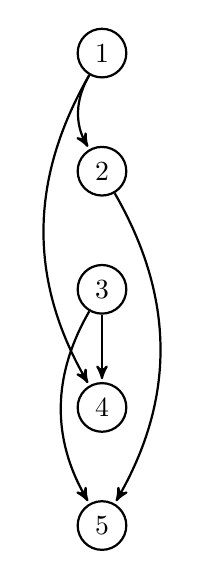
\begin{tikzpicture}[->,>=stealth',shorten >=1pt,auto,node distance=1.5cm,
  thick,main node/.style={circle,draw}]

  \node[main node] (1) {1};
  \node[main node] (2) [below of=1] {2};
  \node[main node] (3) [below of=2] {3};
  \node[main node] (4) [below of=3] {4};
  \node[main node] (5) [below of=4] {5};

  \path[every node/.style={font=\sffamily\small}]
    (1) edge [bend right] node [above] {} (4)
        edge [bend right] node [above] {} (2)
    (2) edge [bend left] node [above] {} (5)
    (3) edge node [above] {} (4)
        edge [bend right] node [above] {} (5);

\end{tikzpicture}
\caption{Exemplo de DFG}
\end{figure}


%eopc
%-------------------------------------------------------------------------------
%\section{Subcapítulo}




% vim: set ai tw=80 fileencoding=utf8: 
%-------------------------------------------------------------------------------

\chapter{Depêndencia}

Quando um programador escreve um programa em uma linguagem sequêncial, o
resultado esperado será obtido pela execução da primeira linha, depois a segunda
e assim em diante, considerando exceções de controles de fluxos como
\textit{loops} e ramificações. 
Uma vez que o programador especificou a ordem que ele espera que as computações 
sejam realizadas. 
Obter paralelismo de um programa respeitando a estas especificações não é
possível, uma vez que obter paralelismo implica em alterar a ordem das
operações realizadas.

Paralelizar um programa sequêncial significa encontrar uma ordem de execução
diferente da especificada e que irá sempre computar o mesmo resultado.
A programação sequêncial introduz restrições que podem ser críticas para o
resultado esperado do programa, assim para transformar um programa em paralelo é
importante encontrar as restrições menos críticas e realizar transformações para
que o programa continue retornando o resultado correto para qualquer entrada.

%Neste capítulo serão apresentadas uma série de restrições, chamadas de
%dependências que serão necessárias para garantir que as transformações
%realizadas nos programas não afetem o resultado e o significado das computações
%realizadas pelo programa.

Uma dependência é uma relação entre duas declarações no programa. 
Um par de declarações $<S_1,S_2>$ está em uma relação se $S_2$ é executada 
depois de $S_1$ em um programa sequêncial, e deve ser executada após $S_1$ 
em qualquer reordenação válida do programa se a ordem de acesso a 
memória será preservada.

\begin{verbatim}
S1   PI = 3.14159
S2   R = 5 
S3   AREA = PI * R * R
\end{verbatim}

Os resultados obtidos por estas declarações são definidas por aqueles obtidos
quando a ordem da execução realizada seja $<S_1,S_2,S_3>$. 
No entanto nada neste trecho de código torna obrigatório a execução de 
$S_2$ depois de $S_1$, desta forma, os resultados obtidos pela ordem de execução 
$<S_2,S_1,S_3>$ serão os mesmos para a variável $AREA$, seja qual for o valor 
da entrada.
Por outro lado, o momento de execução de $S_3$ é mais crítico, se $S_3$ for
executada antes de $S_1$ ou de $S_2$, os resultados obtidos por esta execução
diferenciariam dos resultados obtidos das computações realizadas na ordem
original.
Em termos de dependência pode-se observar que os pares $<S_1,S_3>$ e $<S_2,S_3>$
estão em uma relação de dependência, embora o par $<S_1,S_2>$ não.
Dependências desse tipo são ditas dependência de dados.

Dependência em linhas de código sequêncial como visto anteriormente, é um
conceito simples de entender.
O problema é que examinar somente linhas de códigos sequênciais não garante 
eficiência em termos de paralelismo. 
Para se obter tal eficiência deve-se considerar os trechos de
código que são mais executados, ou seja, devemos expandir o conceito de
dependência para \textit{loops} e vetores.
O trecho de código a seguir ilustra a complexidade introduzida ao expandirmos o
conceito de dependência.

\begin{verbatim}
        for (int I = 1; I < N; I++){
S1          A[I]   = B[I] + 1;
S2          B[I+1] = A[I] - 5;
        }
\end{verbatim}

Este \textit{loop} mostra a dependência entre $<S_1,S_2>$, uma vez que o
resultado computado de $A$ é imediatamente utilizando por $S_2$ em todas as
iterações, e também a dependêndia entre $<S_2,S_1>$ exceto na primeira iteração,
uma vez que o resultado obtido por $S_2$ será utilizado na iteração anterior.
Detectar estas dependências é difícil, considerando que cada iteração acessa 
diferentes elementos do vetor.

\textit{Loops} e vetores são apenas parte do problema que envolve a análise de
dependência, deve-se considerar também as estruturas condicionais, como as
declarações $IF$.

Deve-se então entender um outro tipo de dependência, dado o trecho de
código a seguir:

\begin{verbatim}
S1     if(d != 0)
S2           a = a / d;
\end{verbatim}

A declaração $S2$ não pode ser executada antes de $S1$, uma vez que essa
transformação pode ocasionar em uma divisão por zero, o que não ocorreria no
programa original. Essa dependência é chamada de dependência de controle.


%referencia: ocfma
%-------------------------------------------------------------------------------



% vim: set ai tw=80 fileencoding=utf8: 
%-------------------------------------------------------------------------------
\section{Dependência de Dados}

Em dependência de dados deve-se garantir que um dado seja produzido e consumido
na ordem correta, assim, cuidando para que não se intercale a leitura e
escrita em um mesmo local, desta forma, durante a leitura pode-se obter um valor 
errado. Da mesma forma, duas escritas devem ocorrer na ordem correta para que na
próxima leitura seja obtido o valor correto.
Dependência de dados pode ser definida como:

\begin{verbatim}
Definição 1: Existe dependência de dados da declaração S1 para a declaração S2
(declaração S2 depende da declaração S1) se e somente se:
        1 -> Ambas as declarações acessam o mesmo local de memória e ao menos
        umas delas escreverão na memória, e
        2 -> Existe um caminho de execução viável de S1 para S2.
\end{verbatim}

Neste capítulo serão apresentadas várias propriedades em que as dependências 
podem ser classificadas.


\subsection{Classificação de Leitura-Escrita}

Em termos da ordem de leitura-escrita, as dependências podem ocorrer de três
maneiras em um programa:

\begin{alineas}
        \item \textit{True dependence.} Onde uma declaração escreve em um local
        que será lido por uma segunda declaração.
        \begin{verbatim}
        S1    x = ...
        S2    ... = x
        \end{verbatim}
        A dependência garante que $S_2$ irá ler exatamente o que foi computado
        por $S_1$. Esse tipo de dependência é também conhecida por dependência de
        fluxo e é denotada por $S_1 \delta S_2$ (lê-se, $S_2$ depende de $S_1$)

        \item \textit{Antidependence.} Uma primeira declaração le de um local
        onde uma segunda declaração irá escrever.
        \begin{verbatim}
        S1    ... = x
        S2    x = ...
        \end{verbatim}
        Esta dependência previne que a troca entre $S_1$ e $S_2$, qual poderia
        fazer com que $S_1$ utiliza-se o valor computado por $S_2$. Em essência
        essa dependência existe para prevenir uma transformação que introduziria
        uma nova dependência do tipo \textit{true dependence} que de fato não
        existe no programa original. \textit{Antidependence} é denotado $S_1
        \delta^- S_2$ ou $S_1 \delta^{-1} S_2$.

        \item \textit{Output dependence.} Ocorre quando duas declaração escrevem
        em um mesmo local.
        \begin{verbatim}
        S1    x = ...
        S2    x = ...
        \end{verbatim}
        Essa dependência previne que ocorra uma troca em as declarações e faça com
        que uma declaração que irá ler o valor computado não leia o valor
        errado.
        \begin{verbatim}
        S1    x = 1
        S2    ...
        S3    x = 2 
        S4    y = 2 * x
        \end{verbatim}
        \textit{Output dependence} é denotado $S_1 \delta^0 S_2$.
\end{alineas}






%referencia: ocfma
%-------------------------------------------------------------------------------


% vim: set ai tw=80 fileencoding=utf8: 
%-------------------------------------------------------------------------------

\chapter{Reestruturação de Loops}

Na otimização do desempenho de um programa, os maiores ganhos serão obtidos das 
regiões do programa onde gasta-se a mais tempo; as regiões repetitivas do
programa.
Essas correspondem por \textit{loops} iterativos ou funções recursivas.
O foco maior deste trabalho serão os \textit{loops} contáveis, aqueles em que é
possível determinar a quantidade de execuções sem que seja necessário
executa-los.



%-------------------------------------------------------------------------------

% vim: set ai tw=80 fileencoding=utf8: 
%-------------------------------------------------------------------------------

\section{Transformações Simples}

Serão apresentadas algumas transformações simples em \textit{loops} que também
serão utilizadas em outras técnicas apresentadas neste capítulo.

%-------------------------------------------------------------------------------
\subsection{Reordenação das Declarações}

A reordenação pode ser realizada sobre qualquer granularidade, operação,
declaração ou sequência de declarações.

Está técnica pode ser utilizada para vários propósitos. Sendo utilizanda para 
amortizar a latência da memória, melhorar o \textit{data locality} movendo 
declarações ou \textit{loops} que utilizam as mesmas variáveis próximas uma das 
outras e também pode ser utilizada para mover \textit{loops} que estão separados 
para perto um do outro, talvéz permitindo o uso da técnica \textit{loop fusion} 
ou outra técnica.




%-------------------------------------------------------------------------------
\subsection{Unswitching}

\textit{Unswitching} é uma transformação simples que retira do \textit{loop} 
a condição independe do \textit{loop}. 
\textit{Unswitching} trata um \textit{loop} que contenha uma condição e faz com 
que a condição envolva o \textit{loop}. 
A condição deve obrigatoriamente ser independente do \textit{loop}.
A vantagem do uso do textit{unswitching} é reduzir a frequência de execução da 
condição, uma vez que fora retirada do \textit{loop}. 
A desvantagem desta tranformação é o aumento da complexidade da estrutura do 
\textit{loop}, um \textit{loop} contendo apenas um \textit{loop} mais interno,
agora terá dois ou mais \textit{loops} internos. 
Essa desvantagem pode afetar a aplicabilidade de outras técnicas ou
transformações.




%-------------------------------------------------------------------------------
\subsection{Loop Peeling}

\textit{Loop peeling} remove a primeira ou a ultima iteração do \textit{loop} 
em código separado, podendo ser generalizado e realizado mais de uma vez. 
Essa técnica depente de saber se a variável de controle da iteração é estritamente
positiva, caso não o seja deve-se realizar os devidos cuidados. 
\textit{Loop peeling} também pode ser utilizado para retirar partes de código 
que não dependem do \textit{index} do \textit{loop}, assim, executando-os apenas
uma vez.


%-------------------------------------------------------------------------------
\subsection{Index Set Splitting}

\textit{Index set splitting} ou \textit{loop splitting} é uma generalização de 
\textit{loop peeling}. Essa técnica divide o \textit{index set} de um
\textit{loop} em duas partes, replicando o corpo do \textit{loop}
apropriadamente. 
Assim como em \textit{loop peeling} essa técnica é útil para ajudar o percurso
do \textit{loop}, ou para remover condições que testam a variável que controla
as iterações do \textit{loop}.



%-------------------------------------------------------------------------------
\subsection{Scalar Expansion} 

\ldots

% vim: set ai tw=80 fileencoding=utf8: 
%-------------------------------------------------------------------------------

\section{Loop Fusion}

Se dois \textit{loops} são adjacentes e possuem o mesmo limite, estes podem
ser agrupados em um \textit{loop} simples.
Originalmente, esta técnica fora desenvolvida como uma forma de reduzir os
custos de testes e ramificações no código.

Sem os conceitos de dependências de dados, as descrições anteriores de
\textit{loop fusion} eram restritas a \textit{loops} livres de dependências de
dados. 

O desenvolvimento de \textit{deep memory hierarchies} fez com que esta técnica
fosse importante para aproveitar o \textit{memory locality}.
Utilizando \textit{loop fusion} em \textit{loops} que referenciam os mesmos
dados melhoram o \textit{temporal locality}, podendo impactar significativamente  
o desempenho da memória \textit{cache} e da memória virtual.
Outra vantagem do uso de \textit{loop fusion} seria tirar vantagem de otimizações 
escalares mais eficiêntes no corpo do \textit{loop}, uma vez que o mesmo ficou
maior após o \textit{loop fusion}.

O uso desta técnica é legal se toda dependência de dados é preservada. Após a
aplicação do \textit{loop fusion} todas as relações de dependências devem seguir
o fluxo original.




% vim: set ai tw=80 fileencoding=utf8: 
%-------------------------------------------------------------------------------

\subsection{Loop Fission}

Um \textit{loop} simples pode ser quebrado em dois ou mais \textit{loops}
menores, isso é o inverso de \textit{loop fusion}, essa técnica é chamada de
\textit{loop fission} ou \textit{loop distribution}.
\textit{Loop fission} é muito utilizada em máquinas com 
\textit{instruction cache} menores, esta técnica pode ser utilizada para quebrar
grandes \textit{loops} que não seriam suportados pela \textit{cache} em
\textit{loops} menores que caibam na \textit{cache}.
Podendo também melhorar a \textit{memory locality} em casos onde um único
\textit{loop} utiliza vários vetores, assim dividindo estes vetores entre mains 
de um \textit{loop}.

Quando um \textit{loop} é dividido, o \textit{index} ou \textit{induction
variable} será utilizado em cada parte do \textit{loop}. 
Para evitar problemas em saber quando a \textit{induction variable} será
atualizada, pode ser criada uma nova variável que a substitua, assim trocando
todas as referências por esta nova variável.

Antes de aplicar esta técnica, primeiro será construído um grafo de dependência em
nível das declarações do \textit{loop}. 
Caso não haja ciclos no grafo de dependência, então o \textit{loop} poderá ser
divido em cada nó do grafo. 
Em caso de ciclos no grafo, então a abordagem não poderá ser a mesma, pois
violaria a dependência de dados, logo, se dois nós formam um ciclo no grafo,
eles podem ser unidos em um único nó, pois não será possível separa-los.
Se o grafo de dependência for fortemente conectado, então a não será possível a
aplicação de \textit{loop fission}.

A ordem correta dos \textit{loops} após o \textit{loop fission} pode ser
encontrada através de um grafo acíclico condensado do grafo de dependência.
Sendo cada nó no grafo condensado um \textit{loop}.

Considerando o algoritmo~\ref{fission_ex1} com quatro declarações em seu corpo e
quatro vetores. 
O grafo de dependência pode ser visto na figura~\ref{graph_fission_ex1}. 
Como pode-se observar no grafo de dependência, existe um ciclo entre as linhas
$3$ e $4$, sendo assim, não será possível separa-las em diferentes
\textit{loops}, também existe uma dependência entre a linha $2$ com a linha $3$
e da linha $5$ com a $4$.
O grafo condensado na figura~\ref{condensed_graph_fission_ex1} mostra a
ordem em que os \textit{loops} devem estar.
O algoritmo~\ref{fission_ex2} mostra o resultado de \textit{loop fission} sobre
o algoritmo~\ref{fission_ex1}.

\begin{algorithm}
\caption{Algoritmo em que ser quer aplicar \textit{loop fission}}
\label{fission_ex1}
\begin{algorithmic}[1]

\FOR {I = 1 to N} 
\STATE A(I) = A(I) + B(I - 1)
\STATE B(I) = C(I - 1) * X + C
\STATE C(I) = 1 / B(I)
\STATE D(I) = sqrt(C(I))
\ENDFOR

\end{algorithmic}
\end{algorithm}

\begin{figure}
\centering
\label{graph_fission_ex1}
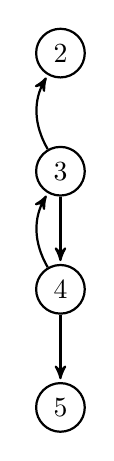
\begin{tikzpicture}[->,>=stealth',shorten >=1pt,auto,node distance=1.5cm,
  thick,main node/.style={circle,draw}]

  \node[main node] (2) {2};
  \node[main node] (3) [below of=2] {3};
  \node[main node] (4) [below of=3] {4};
  \node[main node] (5) [below of=4] {5};

   \path[every node/.style={font=\sffamily\small}]
    (3) edge [bend left] node [below] {} (2)
        edge node [above] {} (4)
    (4) edge [bend left] node [below] {} (3)
        edge node [above] {} (5);

\end{tikzpicture}
\caption{Grafo de dependência do algoritmo~\ref{fission_ex1}}
\end{figure}

\begin{figure}
\centering
\label{condensed_graph_fission_ex1}
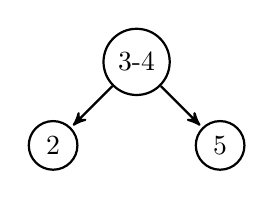
\begin{tikzpicture}[->,>=stealth',shorten >=1pt,auto,node distance=1.5cm,
  thick,main node/.style={circle,draw}]

  \node[main node] (3) {3-4};
  \node[main node] (2) [below left of=3] {2};
  \node[main node] (5) [below right of=3] {5};

   \path[every node/.style={font=\sffamily\small}]
    (3) edge node [below left] {} (2)
        edge node [below right] {} (5);

\end{tikzpicture}
\caption{Grafo condensado acíclico do grafo de dependência}
\end{figure}

\begin{algorithm}
\caption{Resultado de \textit{loop fission} sobre o algoritmo~\ref{fission_ex1}}
\label{fission_ex2}
\begin{algorithmic}[1]

\FOR {I = 0 to N - 1} 
\STATE B(I + 1) = C(I) * X + C
\STATE C(I + 1) = 1 / B(I + 1)
\ENDFOR
\FOR {I = 0 to N - 1} 
\STATE A(I + 1) = A(I + 1) + B(I)
\ENDFOR
\FOR {I = 0 to N - 1} 
\STATE D(I + 1) = sqrt(C(I + 1))
\ENDFOR
\STATE I = I + 1
\end{algorithmic}
\end{algorithm}



% vim: set ai tw=80 fileencoding=utf8: 
%-------------------------------------------------------------------------------
\section{Loop Reversal}

Algumas vezes pode-se desejar que um \textit{loop} intere de trás para frente,
ou seja, do final do percurso do \textit{loop} para o início, e isso é chamado
de \textit{loop reversal}.
Caso existe uma relação de dependência, essa relação muda de sentido devido ao
decrescimento do índice do \textit{loop}, com isso violando a relação de 
dependência.

Um uso para esta técnica é permitir o uso de \textit{loop fusion} onde antes não
era permitido. 
Considere o algoritmo~\ref{fusion_dep}, onde a fusão de três \textit{loops}
resultou em dois \textit{loops}, ver algoritmo~\ref{fusion_dep3}. 
Aplicando \textit{loop reversal} pode-se obter apenas um \textit{loop} como
resultado, algoritmo~\ref{reversal_ex}.

\begin{algorithm}
\caption{Resultado da aplicação de \textit{loop reversal} e \textit{loop fusion}
no algoritmo~\ref{fusion_dep3}}
\label{reversal_ex}
\begin{algorithmic}[1]

\FOR {I = N downto 0}
\STATE A(I) = B(I) + 1
\STATE C(I) = A(I) / 2
\STATE D(I) = 1 / C(I + 1)
\ENDFOR

\end{algorithmic}
\end{algorithm}

% vim: set ai tw=80 fileencoding=utf8: 
%-------------------------------------------------------------------------------
\subsection{Loop Interchanging}

\textit{Loop interchanging} talvez seja a mais importante técnica de
reestruturação de \textit{loops}.
Esta técnica resume-se em \textit{loops} que estejam fortemente aninhados
serem trocados de posição, o \textit{loop} mais externo é trocado pelo mais
interno.
No caso de apenas um \textit{loop} carregar todas as dependências, este pode ser
trocado de posição e se tornar o \textit{loop} mais externo, assim, os outros
\textit{loops} podem ser executados em paralelo \cite{hpcfpc}.

\textit{Loop interchanging} tem sido utilizado para melhorar o desempenho 
de um programa.
Um \textit{loop} mais externo com um número maior de iterações e o 
\textit{loop} mais interno com apenas algumas iterações, em um cenário como este
haverá \textit{loop startup overhead} sobre o \textit{loop} mais interno,
trocando-os de posição, a ocorrência de \textit{loop startup overhead} será de
apenas algumas vezes.

%-------------------------------------------------------------------------------
\subsubsection{Loops Fortemente Aninhados}

Dois \textit{loops} estão fortemente aninhados quando o único código no corpo do
\textit{loop} mais externo for o \textit{loop} mais interno.
Para \textit{loops} contáveis, com percurso do \textit{loop} mais interno não
dependendo da iteração do \textit{loop} mais externo, aplicar \textit{loop
interchanging} será apenas troca-los de posição.
Ao aplicar \textit{loop interchanging} no algoritmo~\ref{fortemente_ex1}
seria obtido o algoritmo~\ref{fortemente_ex2} como resultado.

\begin{algorithm}
\caption{Dois \textit{loops} fortemente aninhados}
\label{fortemente_ex1}
\begin{algorithmic}[1]

\FOR {I = }
\FOR {J = }
\STATE corpo do loop
\ENDFOR
\ENDFOR

\end{algorithmic}
\end{algorithm}


\begin{algorithm}
\caption{Resultado de \textit{loop interchanging} no
        algoritmo~\ref{fortemente_ex1}}
\label{fortemente_ex2}
\begin{algorithmic}[1]

\FOR {J = }
\FOR {I = }
\STATE corpo do loop
\ENDFOR
\ENDFOR

\end{algorithmic}
\end{algorithm}

Assim como em todas as técnicas de reestruturação de \textit{loops}, deve-se
atentar em preservar as relações de dependência entre os \textit{loops}. 
Se toda dependência for preservada e o sentido do programa se mantiver, então, o
resultado do \textit{loop interchanging} será sempre válido.


%-------------------------------------------------------------------------------
\subsubsection{Loops Não Fortemente Aninhados}

\textit{Loops} não fortemente aninhados, ao contrário do fortemente aninhado, o
\textit{loop} mais externo tem mais declaração em seu corpo do que apenas o
\textit{loop} interno.
As vezes é  possível  transformar  \textit{loops} não fortemente aninhados em
fortemente aninhados utilizando-se \textit{loop fission}.
Algumas vezes isto pode não ser possível, então outra forma de faze-lo seria
colocar estas declarações do \textit{loop} mais externo dentro do corpo do
\textit{loop} mais interno, utilizando-se de declarações condicionais para
ajustar em qual iteração devem ser executadas. 
Um ajuste possível seria executa-las quando o \textit{index} dos \textit{loops}
forem iguais, outro ajuste seria a criação de uma nova iteração no início ou fim
para executa-las \cite{hpcfpc}.

Utilizando o ajuste condicional de igualdade  do \textit{index} com mesmo limite
de percurso aplicada ao algoritmo~\ref{nf_1}, resultaria no
algoritmo~\ref{nf_2}.

\begin{algorithm}
\caption{Dois \textit{loops} não fortemente aninhados}
\label{nf_1}
\begin{algorithmic}[1]

\FOR {I = 1 to N}
\STATE corpo do loop externo
\FOR {J = 1 to N}
\STATE corpo do loop interno
\ENDFOR
\ENDFOR

\end{algorithmic}
\end{algorithm}

\begin{algorithm}
\caption{Resultado de \textit{loop interchanging} no algoritmo~\ref{nf_1}}
\label{nf_2}
\begin{algorithmic}[1]

\FOR {J = 1 to N}
\FOR {I = 1 to N}
\IF {I == J}
\STATE corpo do loop externo
\ELSE
\STATE corpo do loop interno
\ENDIF
\ENDFOR
\ENDFOR

\end{algorithmic}
\end{algorithm}




% vim: set ai tw=80 sw=2 fileencoding=utf8: 
%-------------------------------------------------------------------------------
\chapter{Experimentos e Resultados}

Este capítulo apresenta os resultado obtidos na aplicação das técnicas de
transformação de \textit{loops} e também
os experimentos realizados.

Para a realização dos experimentos foi escolhido o programa
\textit{wat\footnote{https://github.com/luizguilhermecm/wat}}, que é um
equalizador de áudio de 1 e 2 canais.

%A escolha de \textit{wat} foi motivado pela fato deste trabalhar com árquivos de
%áudio, ou seja, grandes vetores de dados e \textit{loops} que iterem sobre estes
%dados. 
%Estes \textit{loops} oferecem uma grande chance de ganho de desempenho por
%iterarem um grande número de vezes.
%Ganho de desempenho sobre \textit{wat} resultaria em uma equalização mais rápida.

Á escolha do \textit{wat} foi motivada pelo fato de ser compatível com arquivos 
compostos de grandes vetores de dados. 
Arquivos de áudio apresentam essa composição. 
Sobre esses vetores são iterados \textit{loops} uma grande quantidade de vezes. 
Isso permite que se ganhe desempenho aplicando modificações sobre os loops do 
\textit{wat}. Tal ganho de desempenho resulta em uma equalização mais rápida.

%-------------------------------------------------------------------------------
\section{Experimentos}

Nesta seção serão apresentados os testes e experimentos realizados sobre os
\textit{loops} extraídos de \textit{wat}, assim como seus resultados
individuais. 

\subsection{Experimento 1}
Analisando o \textit{loop} do algoritmo~\ref{read_data_orig} o qual 
transforma dois \textit{bytes} em um \textit{double}.

\begin{algorithm}[H]
  \caption{\textit{Loop} extraído do \textit{wat}.}
    \label{read_data_orig}
\lstinputlisting[language=c]{resultados/src/read_data_orig.c}
\end{algorithm}


Devido a existência de uma declaração \textit{if} no corpo do \textit{loop} e
sendo este \textit{if} independente do \textit{loop}. 
Foi aplicado a técnica \textit{loop unswitching}, que retira a comparação
\textit{if} do corpo do \textit{loop} envolvendo um novo \textit{loop} para cada caso
da comparação, assim nenhum dos \textit{loops} terão declações de comparação em seu
corpo.
O algoritmo~\ref{read_data_opt} mostra o resultado do
algoritmo~\ref{read_data_orig} após a alteração com o uso de \textit{loop unswitching}.

Considerando o algoritmo~\ref{read_data_opt} será aplicado a técnica 
\textit{loop unroll} com o intuito de diminuir o número de iterações e 
consequentemente a
quantidade de comparações realizadas no \textit{loop} em duas vezes. 
O algoritmo~\ref{read_data_unroll} mostra o resultado do \textit{loop
unroll} duplicando o corpo do \textit{loop}.

Considerando o algoritmo~\ref{read_data_opt} onde o primeiro \textit{loop} itera
sobre dois vetores e o segundo \textit{loop} itera
sobre três vetores, será aplicado \textit{loop fission} dividindo-os de forma
que cada \textit{loop} itere somente sobre um vetor.
O algoritmo~\ref{read_data_fission} mostra o resultado de \textit{loop fission}
no algoritmo~\ref{read_data_opt}.

O algoritmo~\ref{read_data_fission} apresenta cinco \textit{loops}, cada um
iterando sobre um vetor. Será aplicado \textit{loop unrolling} dobrando o corpo
de cada um dos \textit{loops} para que o número de iterações seja dividido por
dois.
O algoritmo~\ref{read_data_unrofis} mostra o resultado de \textit{loop
unrolling} no algoritmo~\ref{read_data_fission}.

A tabela~\ref{tabela_read_data} apresenta os resultados obtidos sobre o
algoritmo~\ref{read_data_orig}.

\begin{table}[H]
  \caption{Resultados das técnicas sobre o algoritmo~\ref{read_data_orig}.}
  \label{tabela_read_data}
\begin{center}
  \begin{tabular}{c|c|c}
    Algoritmo & Técnicas aplicadas & Tempo de execução\\
    \hline
    Algoritmo~\ref{read_data_orig} & nenhuma & 111 \textit{ms} \\
    \hline
    Algoritmo~\ref{read_data_opt} & \textit{loop unswitching} & 111 \textit{ms} \\
    \hline
    Algoritmo~\ref{read_data_unroll} & \textit{loop unswitching, loop unroll} & 221 \textit{ms} \\
    \hline
    Algoritmo~\ref{read_data_fission} & \textit{loop unswitching, loop fission} & 111 \textit{ms} \\
    \hline
  Algoritmo~\ref{read_data_unrofis} & \textit{loop unswitching, loop fisson, loop unroll} & 111 \textit{ms} \\
    \hline
  \end{tabular}
\end{center}
\end{table}


\begin{algorithm}[H]
  \caption{\textit{Loop unswitching} no algoritmo~\ref{read_data_orig}.}
    \label{read_data_opt}
\lstinputlisting[language=c]{resultados/src/read_data_opt.c}
\end{algorithm}

\begin{algorithm}[H]
  \caption{\textit{Loop unroll} no algoritmo~\ref{read_data_opt}.}
    \label{read_data_unroll}
\lstinputlisting[language=c]{resultados/src/read_data_unroll.c}
\end{algorithm}

\begin{algorithm}[H]
  \caption{\textit{Loop fission} no algoritmo~\ref{read_data_opt}.}
    \label{read_data_fission}
\lstinputlisting[language=c]{resultados/src/read_data_fission.c}
\end{algorithm}

\begin{algorithm}[H]
  \caption{\textit{Loop unrolling} no algoritmo~\ref{read_data_fission}.}
    \label{read_data_unrofis}
\lstinputlisting[language=c, basicstyle=\tiny ]{resultados/src/read_data_unrofis.c}
\end{algorithm}

%-------------------------------------------------------------------------------
\subsection{Experimento 2}

Analisando o \textit{loop} do algoritmo~\ref{fix_data_orig} que rearranja os dados
para o calculo da FFT. 

\begin{algorithm}[H]
  \caption{Loop extraído do \textit{wat}.}
    \label{fix_data_orig}
\lstinputlisting[language=c]{resultados/src/fix_data_orig.c}
\end{algorithm}

O algoritmo~\ref{fix_data_orig} é parecido com o algoritmo~\ref{read_data_orig}, uma
vez que ambos contêm uma declaração \textit{if} independente do \textit{loop} em seu corpo. 
Assim, também foi aplicado a técnica \textit{loop unswitching} no
algoritmo~\ref{fix_data_orig}.
O algoritmo~\ref{fix_data_opt} mostra o resultado da aplicação de \textit{loop
unswitching} no algoritmo~\ref{fix_data_orig}.

Com o intuito de diminuir o número de iterações será aplicado \textit{loop
unroll} no algoritmo~\ref{fix_data_opt}. 
O algoritmo~\ref{fix_data_unroll} mostra o resultado de \textit{loop unroll} no
algoritmo~\ref{fix_data_opt}.

Considerando o algoritmo~\ref{fix_data_opt} onde o segundo \textit{loop} itera
sobre dois vetores. Será aplicado \textit{loop fission}, dividindo-o em dois 
\textit{loops} onde cada um itere em um vetor.
O algoritmo~\ref{fix_data_fission} mostra o resultado de \textit{loop fission}
no algoritmo~\ref{fix_data_opt}.

Com algoritmo~\ref{fix_data_fission} agora com três \textit{loops}. Será
aplicado \textit{loop unrolling} neste para que o número de iterações em cada
\textit{loop} seja dividido por dois. 
O algoritmo~\ref{fix_data_unrofis} mostra o resultado de \textit{loop unrolling}
no algoritmo~\ref{fix_data_fission}.

A tabela~\ref{tabela_fix_data} apresenta os resultados obtidos sobre o
algoritmo~\ref{fix_data_orig}.

\begin{table}[H]
  \caption{Resultados das técnicas sobre o algoritmo~\ref{fix_data_orig}.}
  \label{tabela_fix_data}
\begin{center}
  \begin{tabular}{c|c|c}
    Algoritmo & Técnicas aplicadas & Tempo de execução\\
    \hline
    Algoritmo~\ref{fix_data_orig} & nenhuma & 111 \textit{ms} \\
    \hline
    Algoritmo~\ref{fix_data_opt} & \textit{loop unswitching} & 111 \textit{ms} \\
    \hline
    Algoritmo~\ref{fix_data_unroll} & \textit{loop unswitching, loop unroll} & 221 \textit{ms} \\
    \hline
    Algoritmo~\ref{fix_data_fission} & \textit{loop unswitching, loop fission} & 111 \textit{ms} \\
    \hline
  Algoritmo~\ref{fix_data_unrofis} & \textit{loop unswitching, loop fisson, loop unroll} & 111 \textit{ms} \\
    \hline
  \end{tabular}
\end{center}
\end{table}



\begin{algorithm}[H]
  \caption{\textit{Loop unswitching} no algoritmo~\ref{fix_data_orig}.}
    \label{fix_data_opt}
\lstinputlisting[language=c]{resultados/src/fix_data_opt.c}
\end{algorithm}

\begin{algorithm}[H]
  \caption{\textit{Loop unroll} no algoritmo~\ref{fix_data_opt}.}
    \label{fix_data_unroll}
\lstinputlisting[language=c]{resultados/src/fix_data_unroll.c}
\end{algorithm}

\begin{algorithm}[H]
  \caption{\textit{Loop fission} no algoritmo~\ref{fix_data_opt}.}
    \label{fix_data_fission}
\lstinputlisting[language=c]{resultados/src/fix_data_fission.c}
\end{algorithm}

\begin{algorithm}[H]
  \caption{\textit{Loop unrolling} no algoritmo~\ref{fix_data_fission}.}
    \label{fix_data_unrofis}
\lstinputlisting[language=c]{resultados/src/fix_data_unrofis.c}
\end{algorithm}

%%-------------------------------------------------------------------------------
\subsection{Experimento 3}

Analisando o \textit{loop} do algoritmo~\ref{equalize_orig} o qual multiplica um dado 
vetor por onze fatores de equalização.

\begin{algorithm}[H]
  \caption{\textit{Loop} extraído do \textit{wat}.}
\label{equalize_orig}
\lstinputlisting[language=c]{resultados/src/equalize_orig.c}
\end{algorithm}

O algoritmo~\ref{equalize_orig} também possui declaração de comparação no corpo do
\textit{loop}, porém as comparações do algoritmo~\ref{equalize_orig} dependem da
iteração do \textit{loop}, sendo assim não é permitido a aplicação de
\textit{loop unswitching}.

Para este \textit{loop} foi aplicado a técnica \textit{index set
splitting}, uma vez que os limites do \textit{loop} e também o valor de cada
comparação realizada ser fixo no programa, o \textit{index set splitting} irá
dividir o \textit{loop} em onze \textit{loops} com o espaço de iteração variando
de \textit{BAND\_MIN} até \textit{BAND\_0}, \textit{BAND\_0} até \textit{BAND\_1} e
assim até o ultimo \textit{loop} que irá iterar de \textit{BAND\_9} até
\textit{BAND\_MAX}. Com isso será eliminado todas as declarações de comparação e
continuará iterando o mesmo número de vezes.

O algoritmo~\ref{equalize_opt} mostra o resultado da aplicação de 
\textit{index set splitting} no algoritmo~\ref{equalize_orig}.

Com o intuito de diminuir o número de iterações no algoritmo~\ref{equalize_opt}
foi aplicado \textit{loop unrolling} em cada um dos onze \textit{loops}. 
O algoritmo~\ref{equalize_unroll} mostra o resultado de \textit{loop unrolling}
no algoritmo~\ref{equalize_opt}.

A tabela~\ref{tabela_equalize} apresenta os resultados obtidos sobre o
algoritmo~\ref{equalize_orig}.

\begin{table}[H]
  \caption{Resultados das técnicas sobre o algoritmo~\ref{equalize_orig}.}
  \label{tabela_equalize}
\begin{center}
  \begin{tabular}{c|c|c}
    Algoritmo & Técnicas aplicadas & Tempo de execução\\
    \hline
    Algoritmo~\ref{equalize_orig} & nenhuma & 111 \textit{ms} \\
    \hline
    Algoritmo~\ref{equalize_opt} & \textit{index set splitting} & 111 \textit{ms} \\
    \hline
    Algoritmo~\ref{equalize_unroll} & \textit{index set splitting, loop unroll} & 221 \textit{ms} \\
    \hline
  \end{tabular}
\end{center}
\end{table}



\begin{algorithm}[H]
  \caption{\textit{Index set splitting} no algoritmo~\ref{equalize_orig}.}
\label{equalize_opt}
\lstinputlisting[language=c]{resultados/src/equalize_opt.c}
\end{algorithm}

\begin{algorithm}[H]
  \caption{\textit{Loop unrolling} no algoritmo~\ref{equalize_opt}.}
\label{equalize_unroll}
\lstinputlisting[language=c, basicstyle=\tiny]{resultados/src/equalize_unroll.c}
\end{algorithm}

%%-------------------------------------------------------------------------------
\subsection{Experimento 4}

Analisando o \textit{loop} do algoritmo~\ref{back_data_orig} que transforma os 
dados após a aplicação da FFT.

\begin{algorithm}[H]
  \caption{\textit{Loop} extraído do \textit{wat}.}
\label{back_data_orig}
\lstinputlisting[language=c]{resultados/src/back_data_orig.c}
\end{algorithm}

O algoritmo~\ref{back_data_orig} também contém uma declaração \textit{if} no corpo do
\textit{loop} que é independente do \textit{loop}. Assim, foi também
aplicado neste \textit{loop} a técnica \textit{loop unswitching}.
O algoritmo~\ref{back_data_opt} mostra o resultado de \textit{loop unswitching} no
algoritmo~\ref{back_data_orig}.

Para que o número de iteração no algoritmo~\ref{back_data_opt} diminua foi
aplicado \textit{loop unrolling}. O algoritmo~\ref{back_data_unroll} mostra o
resultado de \textit{loop unrolling} no algoritmo~\ref{back_data_orig}.

O segundo \textit{loop} do algoritmo~\ref{back_data_opt} está iterando sobre dois
vetores do lado direito das declarações de atribuição, sendo assim, foi
aplicado \textit{loop fission}, dividindo-os em dois \textit{loops}.
O algoritmo~\ref{back_data_fission} mostra o resultado de \textit{loop fission}
no algoritmo~\ref{back_data_opt}.

Para diminuir o número de iterações dos \textit{loops} do
algoritmo~\ref{back_data_fission} foi aplicado \textit{loop unrolling} em cada um
dos \textit{loops}. O algoritmo~\ref{back_data_unrofis} mostra o resultado de
\textit{loop unrolling} no algoritmo~\ref{back_data_fission}.


A tabela~\ref{tabela_back_data} apresenta os resultados obtidos sobre o
algoritmo~\ref{back_data_orig}.

\begin{table}[H]
  \caption{Resultados das técnicas sobre o algoritmo~\ref{back_data_orig}.}
  \label{tabela_back_data}
\begin{center}
  \begin{tabular}{c|c|c}
    Algoritmo & Técnicas aplicadas & Tempo de execução\\
    \hline
    Algoritmo~\ref{back_data_orig} & nenhuma & 111 \textit{ms} \\
    \hline
    Algoritmo~\ref{back_data_opt} & \textit{loop unswitching} & 111 \textit{ms} \\
    \hline
    Algoritmo~\ref{back_data_unroll} & \textit{loop unswitching, loop unroll} & 221 \textit{ms} \\
    \hline
    Algoritmo~\ref{back_data_fission} & \textit{loop unswitching, loop fission} & 111 \textit{ms} \\
    \hline
  Algoritmo~\ref{back_data_unrofis} & \textit{loop unswitching, loop fisson, loop unroll} & 111 \textit{ms} \\
    \hline
  \end{tabular}
\end{center}
\end{table}



\begin{algorithm}[H]
\caption{\textit{Loop unswitching} no algoritmo~\ref{back_data_orig}.}
\label{back_data_opt}
\lstinputlisting[language=c]{resultados/src/back_data_opt.c}
\end{algorithm}


\begin{algorithm}[H]
\caption{\textit{Loop unrolling} no algoritmo~\ref{back_data_opt}.}
\label{back_data_unroll}
\lstinputlisting[language=c]{resultados/src/back_data_unroll.c}
\end{algorithm}

\begin{algorithm}[H]
\caption{\textit{Loop fission} no algoritmo~\ref{back_data_opt}.}
\label{back_data_fission}
\lstinputlisting[language=c]{resultados/src/back_data_fission.c}
\end{algorithm}

\begin{algorithm}[H]
\caption{\textit{Loop unrolling} no algoritmo~\ref{back_data_fission}.}
\label{back_data_unrofis}
\lstinputlisting[language=c]{resultados/src/back_data_unrofis.c}
\end{algorithm}
%%-------------------------------------------------------------------------------
\subsection{Experimento 5}

Analisando o algoritmo~\ref{convert_double_orig} que apresenta 
dois \textit{loops},
sendo que o primeiro converte um vetor \textit{double} em um vetor 
\textit{short int} e o segundo \textit{loop} combina os \textit{bytes} do vetor
\textit{short int} em um vetor \textit{unsigned char}.

\begin{algorithm}[H]
  \caption{\textit{Loop} extraído do \textit{wat}.}
\label{convert_double_orig}
\lstinputlisting[language=c]{resultados/src/convert_double_orig.c}
\end{algorithm}

O algoritmo~\ref{convert_double_orig} contém uma declaração \textit{if} no corpo de
cada um dos \textit{loops}, onde ambos são independentes de seu respectivo \textit{loop}. 
Sendo assim, foi aplicada a técnica \textit{loop unswitching} em cada um dos
\textit{loops} do algoritmo~\ref{convert_double_orig} e resultando no
algoritmo~\ref{convert_double_opt}.

O algoritmo~\ref{convert_double_opt} agora sem declaração \textit{if} no corpo
do \textit{loops} apresenta dois \textit{loops} para cada resultado de
\textit{if} ou \textit{else if}, sendo assim, foi feito uma reordenação das
declarações com o intuito de melhorar a legibilidade do código para aplicação de
outras técnicas.
O algoritmo~\ref{convert_double_reo} mostra o resultado da reordenação das
declarações do algoritmo~\ref{convert_double_opt}, onde cada resultado das
comparações possuem dois \textit{loops}, a ordem de computação dos
\textit{loops} foi mantida para que o significado do programa não se altere.

Analisando o algoritmo~\ref{convert_double_reo}, nota-se que os 
\textit{loops} tem como
espaço de iteração o valor de \textit{wi->nb\_samples}, embora o segundo
\textit{loop} itere sobre \textit{wi->nb\_samples * iterator},  é possível aplicar
a técnica \textit{loop fusion} nos \textit{loops}, assim unindo-os em um
único \textit{loop}, sendo necessário ajustar o espaço de iteração. 
Devido ao
segundo \textit{loop} utilizar os dados computados pelo primeiro \textit{loop},
será necessário garantir que essa dependência seja mantida.

A aplicação do \textit{loop fusion} sobre o
algoritmo~\ref{convert_double_opt} pode se tornar confusa devido a aplicação do
\textit{loop unswitching}, que torna mais complexa a leitura do código. 
A reordenação de declarações fez com que o algoritmo~\ref{convert_double_opt}
ficasse mais legível.
O algoritmo~\ref{convert_double_fusion} mostra o 
resultado de \textit{loop fusion} no algoritmo~\ref{convert_double_reo}. 

O algoritmo~\ref{convert_double_fusion} apresenta dois \textit{loops}, onde o
segundo \textit{loop} itera sobre uma cinco vetores com um número de iteração
igual ao número de \textit{bytes} do arquivo de áudio. 
Será aplicado \textit{loop fission} no segundo \textit{loop} com o intuito de
dividi-lo em dois \textit{loops} onde cada um itere sobre um dos canais de
áudio.
O algoritmo~\ref{convert_double_fission} mostra o resultado de \textit{loop
fission} no algoritmo~\ref{convert_double_fusion}.


A tabela~\ref{tabela_convert_double} apresenta os resultados obtidos sobre o
algoritmo~\ref{convert_double_orig}.


\begin{table}[H]
  \caption{Resultados das técnicas sobre o algoritmo~\ref{convert_double_orig}.}
  \label{tabela_convert_double}
\begin{center}
  \begin{tabular}{c|c|c}
    Algoritmo & Técnicas aplicadas & Tempo de execução\\
    \hline
    Algoritmo~\ref{convert_double_orig} & nenhuma & 111 \textit{ms} \\
    \hline
    Algoritmo~\ref{convert_double_opt} & \textit{loop unswitching} & 111 \textit{ms} \\
    \hline
    Algoritmo~\ref{convert_double_fusion} & \textit{loop unswitching, loop fusion} & 221 \textit{ms} \\
    \hline
    Algoritmo~\ref{convert_double_fission} & \textit{loop unswitching, loop fusion, loop fission} & 111 \textit{ms} \\
    \hline
  \end{tabular}
\end{center}
\end{table}



\begin{algorithm}[H]
  \caption{\textit{Loop unswitching} no algoritmo~\ref{convert_double_orig}.}
\label{convert_double_opt}
\lstinputlisting[language=c]{resultados/src/convert_double_opt.c}
\end{algorithm}

\begin{algorithm}[H]
  \caption{Reordenação das declarações do algoritmo~\ref{convert_double_opt}.}
\label{convert_double_reo}
\lstinputlisting[language=c]{resultados/src/convert_double_reo.c}
\end{algorithm}

\begin{algorithm}[H]
  \caption{\textit{Loop fusion} no algoritmo~\ref{convert_double_reo}.}
\label{convert_double_fusion}
\lstinputlisting[language=c]{resultados/src/convert_double_fusion.c}
\end{algorithm}

\begin{algorithm}[H]
  \caption{\textit{Loop fission} no algoritmo~\ref{convert_double_fusion}.}
\label{convert_double_fission}
\lstinputlisting[language=c]{resultados/src/convert_double_fission.c}
\end{algorithm}

%%-------------------------------------------------------------------------------
\subsection{Experimento 6}

Analisando o \textit{loop} do algoritmo~\ref{save_file_orig} que escreve em arquivo o 
vetor \textit{buffer}.

\begin{algorithm}[H]
  \caption{\textit{Loop} extraído do \textit{wat}.}
\label{save_file_orig}
\lstinputlisting[language=c]{resultados/src/save_file_orig.c}
\end{algorithm}

Para diminuir o número de iterações no algoritmo~\ref{save_file_orig} foi
aplicado \textit{loop unrolling}. O algoritmo~\ref{save_file_unroll} mostra o
resultado de \textit{loop unrolling} no algoritmo~\ref{save_file_orig}.

\begin{algorithm}[H]
  \caption{\textit{Loop unrolling} no algoritmo~\ref{save_file_orig}.}
\label{save_file_unroll}
\lstinputlisting[language=c]{resultados/src/save_file_unroll.c}
\end{algorithm}

A tabela~\ref{tabela_save_file} apresenta os resultados obtidos sobre o
algoritmo~\ref{save_file_orig}.


\begin{table}[H]
  \caption{Resultados das técnicas sobre o algoritmo~\ref{save_file_orig}.}
  \label{tabela_save_file}
\begin{center}
  \begin{tabular}{c|c|c}
    Algoritmo & Técnicas aplicadas & Tempo de execução\\
    \hline
    Algoritmo~\ref{save_file_orig} & nenhuma & 111 \textit{ms} \\
    \hline
    Algoritmo~\ref{save_file_unroll} & \textit{loop unrolling} & 221 \textit{ms} \\
    \hline
  \end{tabular}
\end{center}
\end{table}



%\begin{algorithm}
%\caption{Loop com declaração if }
%\label{read_data_2}
%\begin{lstlisting}[language=c]
%
%\end{lstlisting}
%\end{algorithm}

%%-------------------------------------------------------------------------------
\section{Resultados Experimentais}

Analisando todos os \textit{loops} otimizados houve uma melhora na desempenho
destes em um total de XXX \textit{ms}. Considerando o tempo total do programa a
melhora do desempenho passa a não ser tão considerável devido ao fato de o
cálculo da FFT já estar otimizado e nada mais pode ser feito para melhora-lo.

%\lstinputlisting[language=c]{resultados/src/file.c}

% vim: set ai tw=80 fileencoding=utf8: 
%-------------------------------------------------------------------------------
\chapter{Conclusão}

Neste trabalho foi discutido um procedimento de paralelização de tarefas sobre 
um algoritmo pré-existente. 
Inicialmente apresentou-se uma fundamentação teórica com técnicas clássicas de 
paralelização, tanto em \textit{hardware} como em \textit{software}. 
Em seguida, foi descrita com maior profundidade a programação envolvendo 
paralelismo, destacando-se as técnicas transformação de loops.

O objetivo desse trabalho é aplicar técnicas de transformação de \textit{loops} 
em uma aplicação para melhora de seu desempenho. 
A aplicação utilizada foi o programa de equalização de áudio \textit{wat}. 
Embora existam muitas técnicas, a obtenção de benefícios em usá-las é uma 
característica empírica. 
Devido a isso, os resultados obtidos após as alterações, 
mesmo que apresentando maior desempenho, não demonstram vantagem significativa.

Dessa forma, pode-se elencar alguns trabalhos futuros a fim de se chegar em 
resultados mais expressivos do que os aqui obtidos. 
Entre os trabalhos futuros é desejável que se aborde toda a questão de 
transformação de \textit{loops} voltados a uma arquitetura específica. 
Esse tipo de investigação pode ser motivada por possíveis comportamentos 
diferenciados de um mesmo algoritmo conforme a plataforma de 
\textit{hardware}.


% ----------------------------------------------------------
% ELEMENTOS PÓS-TEXTUAIS
% ----------------------------------------------------------
\postextual


% ----------------------------------------------------------
% Referências bibliográficas
% ----------------------------------------------------------
\bibliography{taxonomia-flynn/bib_taxonomia-flynn,2-introducao/bib_introducao,books,memoria/memoria,loops/loops}

\end{document}
